\documentclass[12pt]{article}

% Настройка русского языка и шрифтов
\usepackage[utf8]{inputenc}
\usepackage[russian]{babel}
\usepackage[T2A]{fontenc}

% Математические пакеты
\usepackage{amsmath, amssymb, amsfonts}

% Настройка страницы
\usepackage{geometry}
\geometry{a4paper, margin=0.8in}

% Другие полезные пакеты
\usepackage{hyperref}
\usepackage{booktabs}
\usepackage{enumitem}
\usepackage{longtable}
\usepackage{graphicx}
\usepackage{xcolor}

% Определение стилей для комментариев
\definecolor{commentgray}{rgb}{0.4,0.4,0.4}
\definecolor{antigravityblue}{rgb}{0.0, 0.45, 0.74}

\newcommand{\commentary}[1]{{\small\itshape\color{commentgray} #1}}
\newcommand{\antigravity}[1]{{\small\color{antigravityblue}\textbf{Antigravity:} #1}}

% Настройка ссылок
\hypersetup{
    colorlinks=true,
    linkcolor=blue,
    filecolor=magenta,      
    urlcolor=cyan,
    pdftitle={Глубокий разбор: Кросс-валидация и чистота эксперимента},
}

\title{Глубокий разбор: Кросс-валидация и чистота эксперимента}
\author{Твой персональный гид по ML}
\date{\today}

\begin{document}

\subsection{Что такое кросс-валидация?}
\textbf{Кросс-валидация} — это процедура оценки качества модели, которая позволяет получить надежную оценку того, как алгоритм будет работать на новых, ранее не виденных данных. Она критически важна для сравнения моделей и подбора гиперпараметров.

\subsection{Метод Hold-out}
Самый простой и быстрый способ. Мы делим данные на две части:
\begin{itemize}
    \item \textbf{Train (обучающая)}: на ней модель учится.
    \item \textbf{Test (тестовая/отложенная)}: на ней мы замеряем качество.
\end{itemize}
Обычно используется пропорция \textbf{70/30} или \textbf{80/20}. 

\textbf{Минус}: Оценка сильно зависит от того, \textit{какие именно} объекты попали в тест. Если в тест случайно попали «легкие» объекты, метрика будет завышена.

\subsection{Стратификация (Stratification)}
Это техника, гарантирующая, что \textbf{распределение классов} (или других важных признаков) в тренировочной и тестовой выборках будет одинаковым. 

\textbf{Зачем это нужно?} Если у вас в данных 95\% здоровых пациентов и 5\% больных, при обычном случайном делении в тест могут вообще не попасть больные люди. Модель покажет 100\% точность, просто предсказывая «здоров», но на деле она бесполезна. 

\textbf{Решение}: Стратификация «нарезает» данные так, чтобы и в трейне, и в тесте сохранялись те же 5\% больных.

\begin{figure}[h]
    \centering
    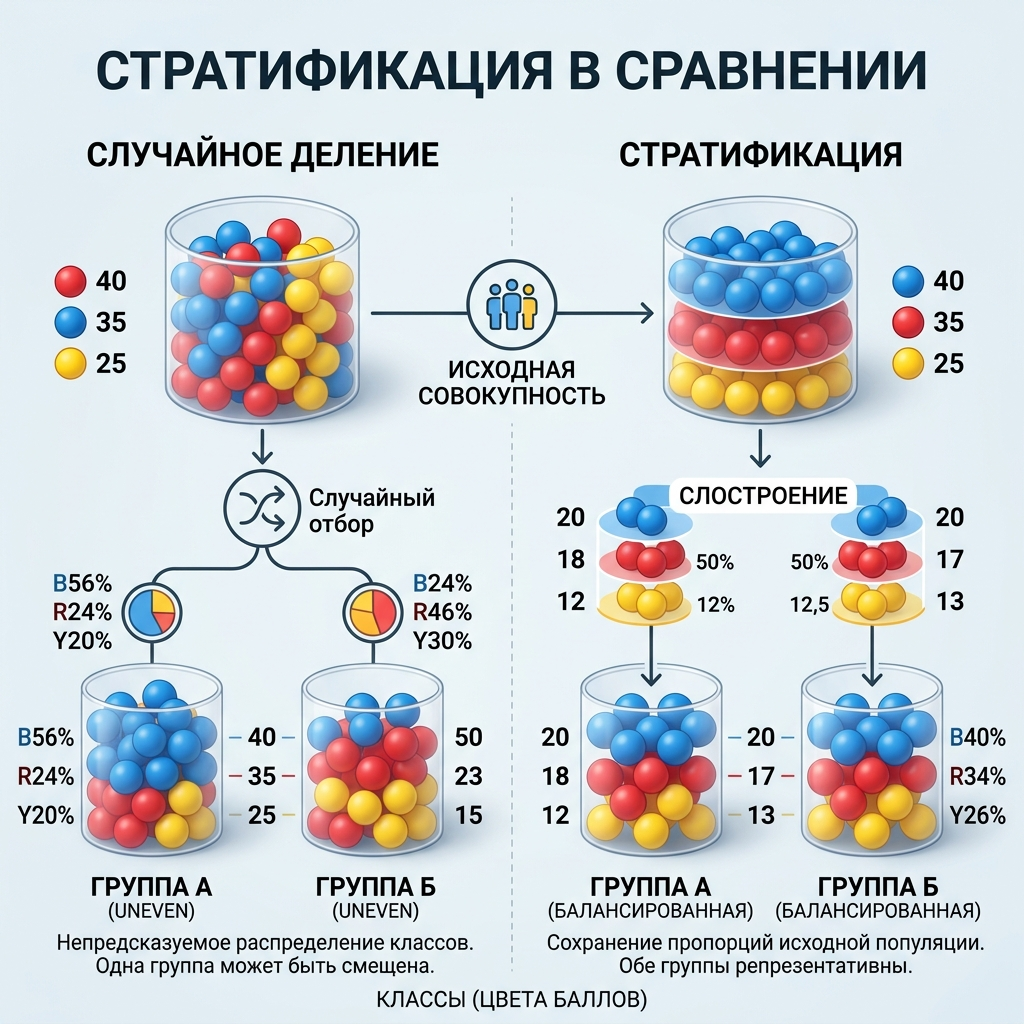
\includegraphics[width=0.7\textwidth]{stratification.png}
    \caption{Визуализация процесса стратификации.}
\end{figure}

\subsection{k-Fold кросс-валидация}
Это «золотой стандарт» оценки. 
\begin{enumerate}
    \item Весь датасет разбивается на $k$ равных частей (фолдов), обычно $k=5$ или $k=10$.
    \item Модель обучается $k$ раз.
    \item На каждой итерации один фолд становится тестовым, а остальные $k-1$ — тренировочными.
    \item Итоговая метрика — это \textbf{среднее арифметическое} результатов всех $k$ итераций.
\end{enumerate}

\begin{figure}[h]
    \centering
    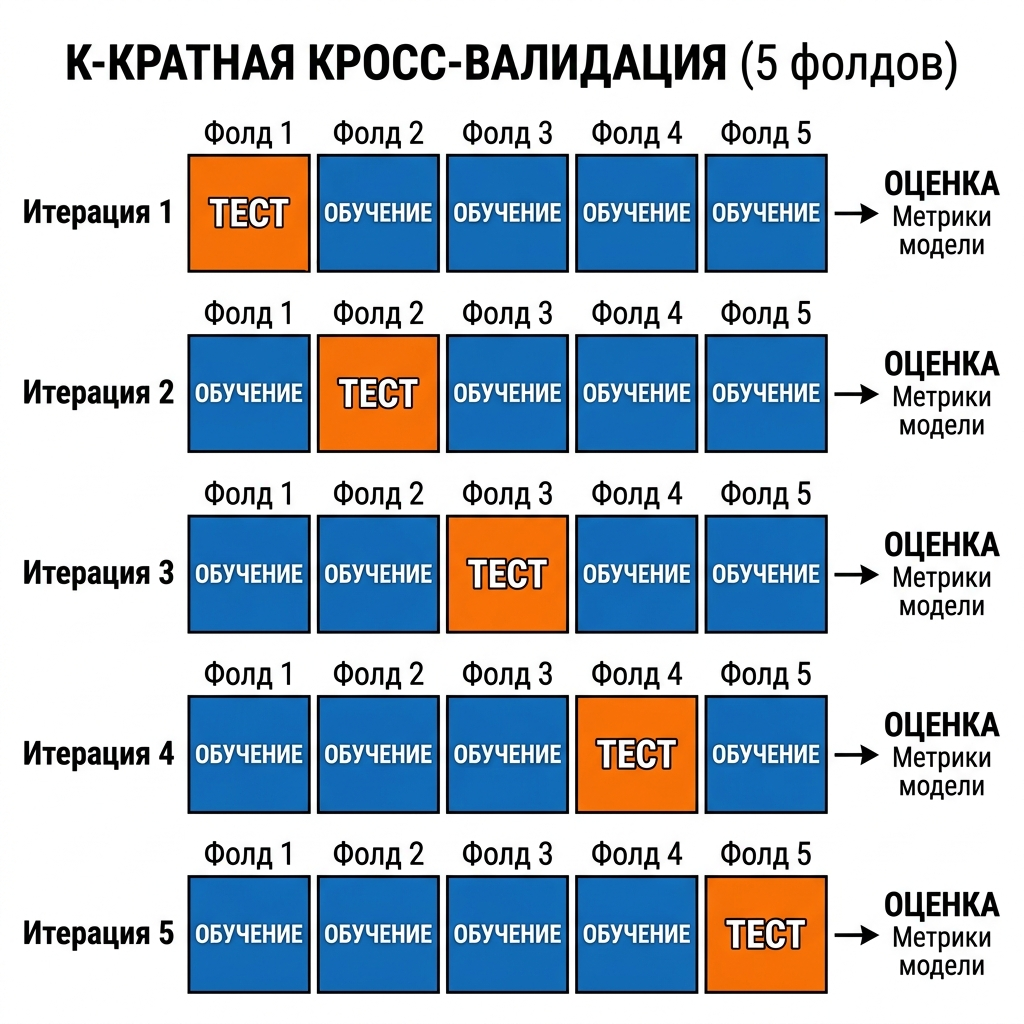
\includegraphics[width=0.7\textwidth]{kfold.png}
    \caption{Схема k-Fold кросс-валидации.}
\end{figure}

\subsection{Leave-one-out (LOO)}
Экстремальный случай k-Fold, где $k$ равно количеству объектов в выборке ($N$).
\begin{itemize}
    \item \textbf{Как это работает}: Мы обучаемся на всех объектах, кроме одного, и на этом одном тестируемся. И так $N$ раз.
    \item \textbf{Плюс}: Мы используем максимум данных для обучения.
    \item \textbf{Минус}: Это невероятно долго и дорого в плане вычислений (если у вас миллион объектов, придется обучить модель миллион раз).
\end{itemize}

\subsection{Stratified k-Fold}
Это комбинация двух методов: данные разбиваются на $k$ фолдов, но при этом в каждом фолде соблюдается \textbf{стратификация}. 
Это самый надежный способ оценки для задач классификации, особенно когда один класс встречается реже другого.

\subsection{Кривые обучения (Learning Curves)}
Перед внедрением найденную лучшую модель можно обучить на всех имеющихся данных. Правда, вы не сможете оценить качество получившейся модели, так как у вас уже не будет тестового множества. Чтобы примерно оценить, как будет вести себя модель при добавлении новых данных, вы можете построить \textbf{кривые обучения}: зависимость качества модели на трейне и на тесте от числа поданных семплов на вход. Это помогает понять, поможет ли сбор дополнительных данных улучшить модель (высокий variance) или модель уперлась в свой предел (высокий bias).

\subsection{Когда стоит заподозрить, что оценка качества завышена?}
Если вы видите метрику \textbf{0.999} или резкий скачок качества по сравнению с бейслайном, не спешите открывать шампанское. Скорее всего, произошел \textbf{Overfitting} или \textbf{Data Leakage}.

\textbf{Красные флаги:}
\begin{enumerate}
    \item Метрика на тесте почти такая же идеальная, как на трейне (для сложных задач это редкость).
    \item Модель отлично работает на кросс-валидации, но «разваливается» на новых реальных данных.
    \item В данных есть признак, который подозрительно сильно коррелирует с таргетом (возможно, это таргет в другом обличии).
\end{enumerate}

\subsection{Примеры «подмешивания» тестовых данных (Data Leakage)}
Это ситуация, когда информация из будущего или из теста просачивается в обучение. Модель «подсматривает» правильные ответы.

\begin{figure}[h]
    \centering
    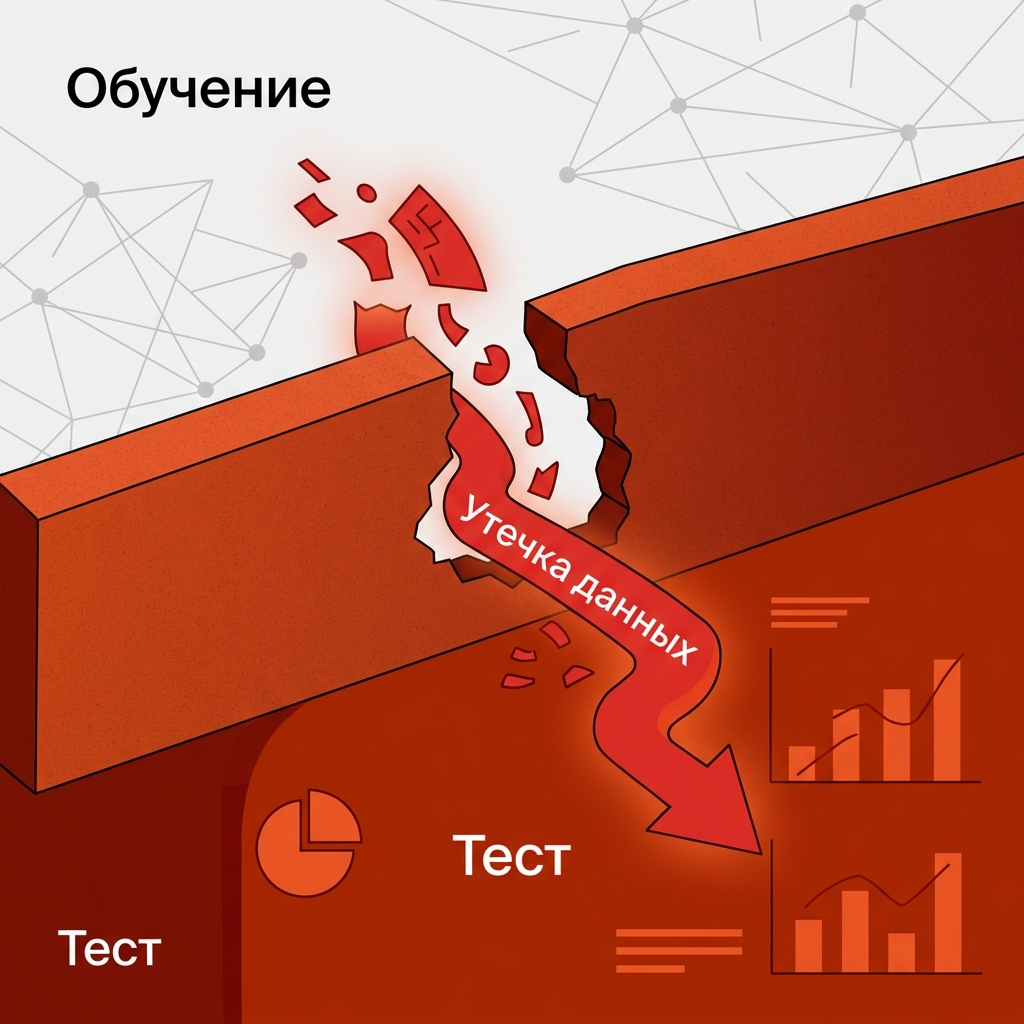
\includegraphics[width=0.6\textwidth]{leakage.png}
    \caption{Схематичное представление утечки данных.}
\end{figure}

\textbf{Примеры:}
\begin{itemize}
    \item \textbf{Масштабирование (Scaling) до разбиения}: Вы посчитали среднее и дисперсию по \textit{всему} датасету, а потом применили \texttt{StandardScaler}. Модель уже «знает» среднее значение тестовой выборки. \textbf{Правильно}: считать параметры только на трейне.
    \item \textbf{Временные ряды (Time Series)}: Вы предсказываете курс акций сегодня, используя данные за завтра. Кросс-валидация моделей для такой задачи осложняется тем, что данные не должны пересекаться по времени: тренировочные данные должны идти до валидационных, а валидационных — до тестовых. С учётом этих особенностей фолды в кросс-валидации для временных рядов располагаются вдоль временной оси (например, метод \textit{Time Series Split} или «скользящее окно»).
    \item \textbf{Дубликаты}: Если в данных есть дублирующиеся строки, один и тот же объект может попасть и в трейн, и в тест. Модель просто «вспомнит» ответ.
    \item \textbf{Косвенные признаки}: Например, предсказание вероятности рака, используя признак «прошел ли пациент химиотерапию». Терапия назначается \textit{после} диагноза, поэтому она содержит ответ в себе.
\end{itemize}

\vspace{1cm}
\commentary{Помни, кросс-валидация — это твой страховой полис. Лучше потратить время на обучение 5 фолдов сейчас, чем через месяц объяснять заказчику, почему «идеальная» модель на практике выдает случайные числа.}

\antigravity{Всегда используй пайплайны. Это защитит тебя от 90\% случаев утечки данных через предобработку.}

\end{document}
